% ══════════════════════════════════════════════════════════════════════
% CHAPTER 4: DATA PROCESSING & GEOSPATIAL ENGINE
% ══════════════════════════════════════════════════════════════════════

\chapter{Data Processing and Geospatial Engine}
\label{ch:data}

This chapter details the processing pipeline that transforms raw seismic observations (whether sourced from local catalogs or remote web services) into optimized, GPU-ready structures for interactive 3D and 4D visualization.

\section{CSV Ingestion and Schema Detection}
\label{sec:csv-ingestion}

\revised{The \texttt{core/loader.py} module handles different formats through an ingestion pipeline that checks the header line for semicolon (\texttt{;}) or comma (\texttt{,}) delimiters, supporting European standards (INGV) as well as international formats (USGS, ISC). To avoid manual preprocessing, \texttt{core/config.py} defines an alias dictionary:}

\begin{lstlisting}[language=Python, caption={Flexible column schema definition in \texttt{core/config.py}.}, label={lst:schema}]
CSV_SCHEMA = {
    'time':  ['time', 'date', 'datetime', 'utc', 'time_utc', 'origintime'],
    'lat':   ['lat', 'latitude'],
    'lon':   ['lon', 'longitude'],
    'depth': ['depth', 'depth_km'],
    'mag':   ['mag', 'magnitude', 'md', 'ml', 'mw']
}
\end{lstlisting}

The ingestion pipeline identifies data columns by reading their headers. It ignores text case and removes any extra spaces. When a file contains unlabelled columns, the loader assumes a standard INGV column order based on their positions. Date processing is equally robust. The engine tests multiple known formats, covering both standard ISO timestamps and common European layouts.

\section{Data Sanitisation and Validation}
\label{sec:sanitisation}

Following ingestion, records undergo a four-stage sanitisation and validation sequence:
\begin{enumerate}
    \item \textbf{Spatial requirement check}: Rows missing latitude, longitude, or timestamps are discarded immediately.
    \item \textbf{Missing metadata flagging}: Catalogues occasionally omit depth or magnitude. \revised{In seismic analysis, estimating missing depths (such as using the mean value) is avoided because it groups points into artificial horizontal layers, distorting clustering and plane fitting results.} Rather than dropping these records (which removes spatial density) or imputing synthetic values, missing fields are flagged via boolean indicators (\texttt{depth\_is\_missing}, \texttt{mag\_is\_missing}) and assigned sentinel defaults (0.0~km depth and magnitude 0.1).
    \item \textbf{Geographic and depth bounds check}: The system excludes any event with mathematically invalid geographic coordinates (i.e., latitude outside the $\pm 90^\circ$ range or longitude outside the $\pm 180^\circ$ range). Additionally, it discards events with a depth falling outside the realistic geological range of $-10$~km to $800$~km, where negative values are specifically permitted to accommodate earthquakes occurring above sea level within mountains or volcanic edifices.
    \item \textbf{Chronological sorting \& future filtering}: Events with future timestamps are discarded, and the remaining catalog is sorted chronologically to optimize slicing.
\end{enumerate}

\section{Online Data Import: The INGV GOSSIP API}
\label{sec:online-import}

The \texttt{core/online\_importer.py} module interfaces directly with the INGV GOSSIP web service \cite{ingv}, providing high-resolution volcanic monitoring catalogues for Campi Flegrei, Vesuvius, and Ischia:

\begin{figure}[htbp]
\centering
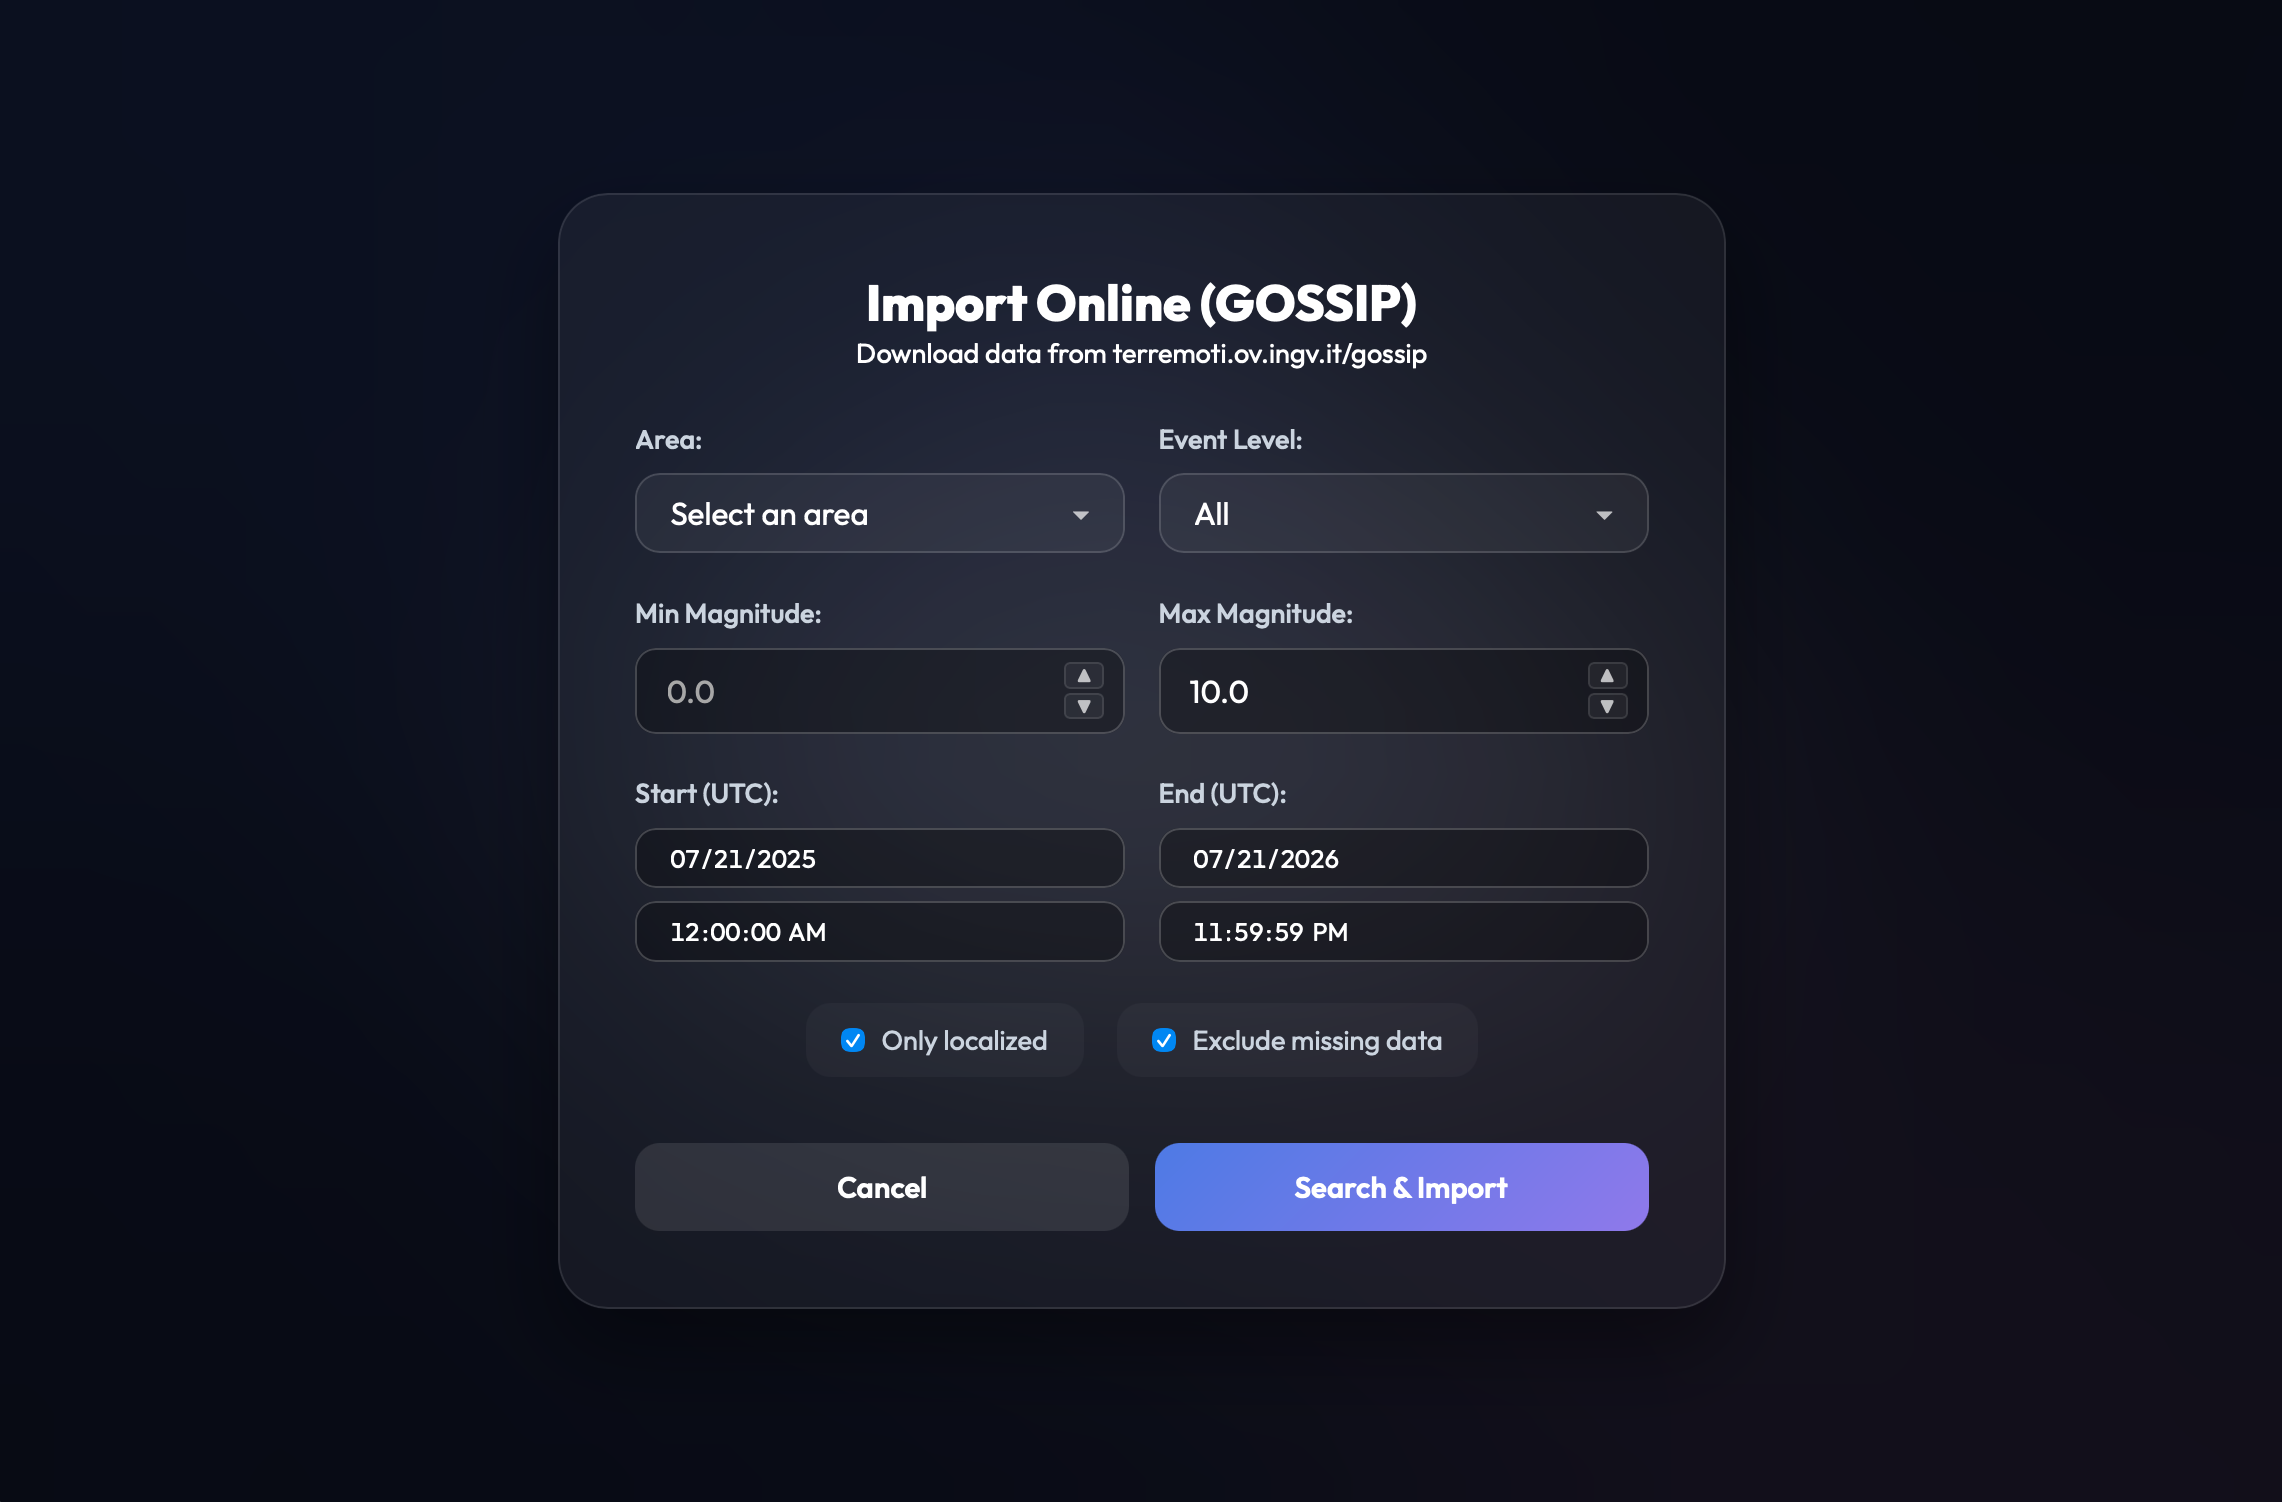
\includegraphics[width=1.0\textwidth]{images/online_import_ingv.png}
\caption{The INGV GOSSIP API import dialog for configuring network criteria, temporal bounds, and quality thresholds.}
\label{fig:online-import-ingv}
\end{figure}

The importer queries the official INGV GOSSIP web portal for each selected year (using the endpoint \texttt{https://\allowbreak terremoti.\allowbreak ov.\allowbreak ingv.\allowbreak it/\allowbreak gossip/\allowbreak <network>/\allowbreak <year>/\allowbreak events.json}). It downloads these annual JSON packets one by one to avoid network failures. As shown in \Cref{fig:online-import-ingv}, users can define the network target, the time span, the magnitude limits ($M_{\min}$ to $M_{\max}$), and the desired INGV revision quality (\texttt{automatico}, \texttt{rivisto}, or \texttt{bollettino}). Users can also apply additional filters to require confirmed coordinates (\texttt{located only}) or to drop records with incomplete information (\texttt{exclude missing}). Finally, the system converts these filtered records into a standard temporary CSV format and forwards them directly to the main ingestion pipeline.

\section{Geospatial Computations and Mesh Generation}
\label{sec:geospatial}

The 3D application visualises seismic activity over a base map retrieved from OpenStreetMap \cite{openstreetmap}. To accurately draw the earthquakes over this map, the software must convert the image pixel positions into standard geographic coordinates. The system solves this problem using an \textbf{inverse Mercator projection} \cite{snyder1987map} (implemented in \texttt{core/geo\_utils.py}). This mathematical operation translates pixel data into latitude and longitude, using NumPy \cite{numpy2020} arrays to guarantee fast execution:
\begin{equation}
    \lambda = \frac{x \cdot s}{t \cdot n} \cdot 360^\circ - 180^\circ, \quad
    \phi = \arctan\left(\sinh\left(\pi \left(1 - \frac{2 \cdot y \cdot s}{t \cdot n}\right)\right)\right) \cdot \frac{180^\circ}{\pi}
    \label{eq:mercator}
\end{equation}
In these equations, $\lambda$ and $\phi$ represent the resulting longitude and latitude in degrees. The values $x$ and $y$ correspond to the horizontal and vertical pixel coordinates on the screen. The variable $s$ is the current scaling factor of the map, while $t$ represents the fixed dimension of a single map tile (256 pixels). Lastly, $n$ is the total number of tiles across the map at the current zoom level $z$, calculated as $n = 2^z$.

\subsection{UTM Zone 33N to WGS84 Conversion}

Some advanced datasets, such as volcanic tomography grids, are originally provided in UTM Zone~33N coordinates instead of standard latitude and longitude. To ensure these layers align correctly with the rest of the 3D map, the \texttt{core/layer\_utils.py} module converts them using a Transverse Mercator inverse projection on the WGS84 ellipsoid:
\begin{equation}
    \phi = \phi_1 - \frac{N_1 \tan\phi_1}{R_1}\left(\frac{D^2}{2} - \frac{(5 + 3T_1 + 10C_1 - 4C_1^2 - 9e'^2)D^4}{24}\right)
\end{equation}
Here, $\phi$ is the final converted latitude. The formula relies on several variables derived from the WGS84 ellipsoid model. Specifically, $\phi_1$ is the footprint latitude, $N_1$ is the prime vertical radius of curvature, and $R_1$ is the meridional radius of curvature at $\phi_1$. The parameter $D$ represents the scaled distance from the central meridian, calculated as $D = (E - 500{,}000) / (N_1 k_0)$, where $E$ is the UTM Easting coordinate and $k_0$ is the central scale factor. Finally, $T_1$, $C_1$, and $e'^2$ are standard geometric constants related to the Earth's eccentricity.

\subsection{Optimised Map Mesh and Caching Architecture}

Terrain generation operates via a five-stage sequence: (1) bounding box squaring for uniform axis resolution, (2) deterministic cache lookup via MD5 hashing of rounded geographic bounds, (3) OpenStreetMap tile downloading via Smopy \cite{smopy} on cache misses, (4) palette-indexed downsampling to $1024 \times 1024$~px (256 colours), and (5) grid transformation via \Cref{eq:mercator}. Meshes are cached both in RAM (\texttt{@lru\_cache(maxsize=4)}) and disk (\texttt{.pkl}), guaranteeing sub-millisecond retrieval on subsequent loads.

\section{Pre-computation and Memory Layout Transformation}
\label{sec:precomputation}
\label{sec:strip-data}
\label{sec:binary-streaming}

To ensure the 3D map remains fluid and responsive even with thousands of earthquakes, the software performs several calculations in advance (during the data loading phase) rather than while the user is interacting with the map. The \texttt{precompute\_visual\_data()} function handles two main tasks. First, it pre-renders tooltip strings in a single batch operation, so that the browser does not need to construct the text for pop-ups every time the mouse hovers over an event. Second, it converts calendar dates into normalised time metrics (days since the first earthquake), accelerating chronological color mapping.

\revised{The data pipeline converts raw CSV lines into contiguous NumPy numerical arrays (\texttt{numpy.ndarray}). This enables vectorised operations on coordinates, depths, and timestamps. To stream data to the client efficiently, arrays are converted to 32-bit floating-point values (\texttt{np.float32}) and transmitted as raw bytes via \texttt{tobytes()}, avoiding JSON encoding overhead.}

\revised{Embedding large amounts of earthquake data directly into an HTML file increases file size and causes the browser to lag. To prevent this, Seismic Viewer uses an asynchronous loading strategy. When the user requests a 3D view, the backend generates an HTML page containing the 3D environment, base terrain maps, and UI menus. Once the base map is displayed, the browser requests the earthquake points in the background via \texttt{/api/data/\{id\}/bin}. These points are delivered as a Float32 binary buffer and populated onto the map without blocking user interaction.}
